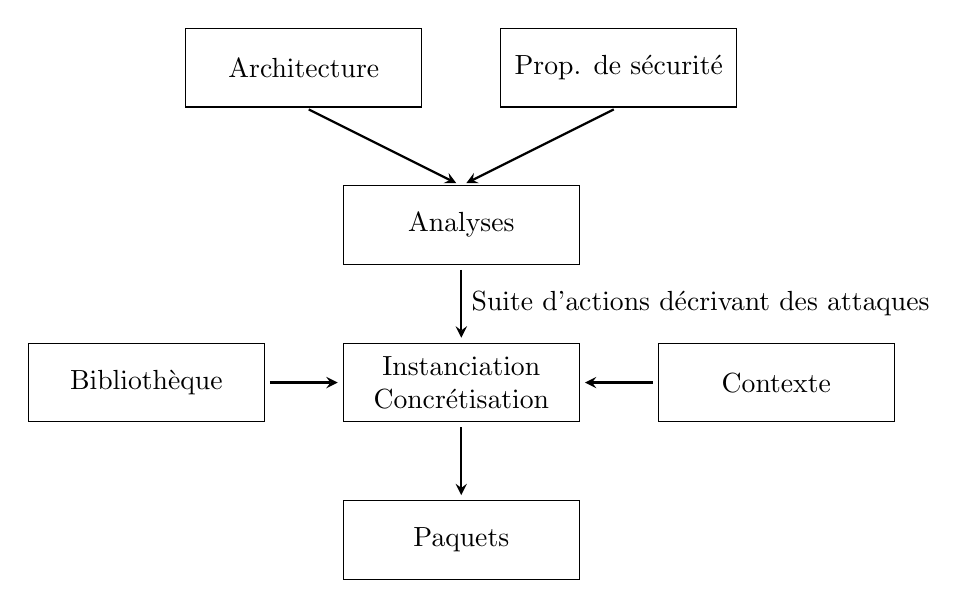
\begin{tikzpicture}[
        arrow/.style={thick,->,shorten >=2pt,shorten <=2pt,>=stealth},
    ]
    \draw (2,6) rectangle (5,7) node [pos=.5] {Architecture};
    \draw (6,6) rectangle (9,7) node [pos=.5] {Prop. de sécurité};


    \draw (4,4) rectangle (7,5) node [pos=.5] {Analyses};

    \draw (0,2) rectangle (3,3) node [pos=.5] {Bibliothèque};
    \draw (4,0) rectangle (7,1) node [pos=.5] {Paquets};
    \draw (8,2) rectangle (11,3) node [pos=.5] {Contexte};

    \draw (4,2) rectangle (7,3) node [align=center,pos=.5] {Instanciation\\Concrétisation};

    \draw[arrow] (3.5,6) -- (5.5,5); % Archi --> Analyses
    \draw[arrow] (7.5,6) -- (5.5,5); % Props --> Analyses
    \draw[arrow] (5.5,4) -- (5.5,3) node [pos=.5,right] {Suite d'actions décrivant des attaques}; % Analyses --> Inst
    \draw[arrow] (3,2.5) -- (4,2.5); % Biblio --> Inst
    \draw[arrow] (8,2.5) -- (7,2.5); % Context--> Inst
    \draw[arrow] (5.5,2) -- (5.5,1); % Inst --> Packets
\end{tikzpicture}
